\documentclass[a4paper,12pt]{article}
\usepackage{amsmath}
\usepackage{graphicx}
\usepackage{geometry}
\usepackage{fancyhdr}
\usepackage{lipsum}
\usepackage{listings}
\usepackage{xcolor}
\usepackage{ragged2e}
\usepackage{hyperref}

\lstset{
    backgroundcolor=\color{gray!10},  
    basicstyle=\ttfamily\footnotesize,  
    numberstyle=\tiny\color{gray},      
    numbersep=5pt,                       
    stepnumber=1,                        
    numberfirstline=true,               
    captionpos=b,                       
    frame=single,                       
    rulecolor=\color{black},            
    breaklines=true,                    
    keywordstyle=\color{blue},          
    commentstyle=\color{green},         
    stringstyle=\color{red},            
    showstringspaces=false,              
    tabsize=2,                          
    numbers=left,                       
    xleftmargin=10pt,                   
    xrightmargin=10pt                   
}


\geometry{top=1in, bottom=1in, left=1.25in, right=1.25in}

\pagestyle{fancy}
\fancyhead[L]{Final Project Pose Estimation - Semaphore Sign Language - PCV}
\fancyhead[R]{2024}

\title{\textbf{Laporan Final Project}\\[1em] \huge Semaphore Sign Language dengan Pose Estimation}
\date{}

\begin{document}

\maketitle

\begin{center}
    
\includegraphics[width=0.6\textwidth]{logo_its.png}
    \vspace{2em}
\end{center}

\begin{center}
  Rigel Ramadhani Waloni \\
  \textbf{5024221058} \\ 
  \vspace{1.5em}
  \textbf{Dosen Pengampu:} \\ 
  Arta Kusuma Hernanda, S.T., M.T. \\ 
  \vspace{3em}
  \textbf{DEPARTEMEN TEKNIK KOMPUTER} \\ 
  FAKULTAS TEKNOLOGI ELEKTRO DAN INFORMATIKA CERDAS \\ 
  INSTITUT TEKNOLOGI SEPULUH NOPEMBER \\ 
  SURABAYA \\
  2024
\end{center}

\newpage

\section[A]{Penjelasan Singkat}
Proyek ini bertujuan untuk menangkap dan menganalisis landmark pose manusia berdasarkan pose semaphore menggunakan pustaka MediaPipe. Sistem ini mendeteksi landmark tubuh manusia menggunakan modul MediaPipe Pose dan menangkap data pose untuk setiap huruf semaphore (A-Z). Data pose yang ditangkap disimpan dalam file JSON di folder \texttt{semaphore\_poses} dan dapat digunakan untuk analisis atau perbandingan lebih lanjut.

Sistem ini menyediakan antarmuka pengguna grafis (GUI) yang dibangun dengan \texttt{customtkinter} untuk memberikan pengalaman yang ramah pengguna. Pengguna dapat memilih gambar dan menyimpan pose yang ditangkap berdasarkan huruf semaphore yang dipilih. Sistem ini juga menyediakan fungsi untuk menguji dan menangkap pose semaphore berdasarkan huruf yang telah ditentukan dan membandingkan pose yang ditangkap dengan yang disimpan dalam file JSON.

\section{Tujuan}
\begin{itemize}
    \item Menganalisis landmark pose manusia berdasarkan pose semaphore menggunakan pustaka MediaPipe.
    \item Menangkap data pose untuk setiap huruf semaphore (A-Z) dan menyimpannya dalam file JSON.
    \item Membangun antarmuka pengguna grafis (GUI) yang ramah pengguna.
    \item Menyediakan fungsi untuk menguji dan menangkap pose semaphore berdasarkan huruf yang telah ditentukan.
    \item Membandingkan pose yang ditangkap dengan yang disimpan dalam file JSON.
\end{itemize}

\section{Teori Singkat}
\subsection{MediaPipe}
MediaPipe adalah kerangka kerja pengolahan media lintas platform yang menyediakan alat dan komponen untuk membangun solusi penglihatan komputer dan pembelajaran mesin. MediaPipe menawarkan berbagai komponen, termasuk deteksi wajah, deteksi pose, pelacakan tangan, dan lainnya. Komponen-komponen ini dapat digunakan untuk membangun aplikasi penglihatan komputer yang beragam, seperti deteksi pose manusia, pelacakan objek, dan lainnya.

\subsection{Pose Estimation}
Pose estimation adalah proses untuk menemukan posisi dan orientasi objek dalam gambar atau video. Pose estimation dapat digunakan untuk mendeteksi pose manusia, pose wajah, pose tangan, dan lainnya. Pose estimation sering digunakan dalam berbagai aplikasi, seperti pengenalan gerakan, analisis gerakan, dan interaksi manusia-mesin.

\subsection{Semaphore Sign Language}
\begin{center}
    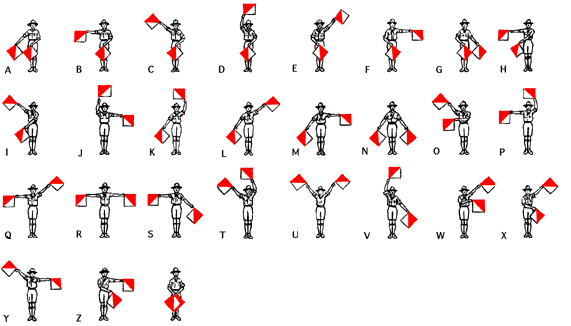
\includegraphics[width=1.0\textwidth]{semaphore.png}
    \vspace{1em}
\end{center}
Semaphore dalam project ini adalah Semaphore Pramuka. Semaphore di pramuka adalah cara komunikasi menggunakan dua bendera yang digerakkan dalam posisi tertentu untuk menyampaikan huruf atau angka. Setiap posisi bendera mewakili simbol atau huruf tertentu, dan digunakan untuk berkomunikasi jarak jauh tanpa suara.

\section{Kode Program dan Penjelasan}
\subsection{Buat Landmark Pose Semaphore dari Gambar dan GUI (get\_landmark.py)}

\begin{lstlisting}[language=Python, caption={Kode Program untuk Mendeteksi Landmark Pose}]
  import cv2
  import mediapipe as mp
  import json
  import os
  import tkinter as tk
  import customtkinter as ctk
  from tkinter import filedialog, messagebox
  from tkinter import ttk
  
  mp_pose = mp.solutions.pose
  mp_drawing = mp.solutions.drawing_utils
  
  landmark_names = {
      0: "nose", 1: "left_eye_inner", 2: "left_eye", 3: "left_eye_outer", 4: "right_eye_inner",
      5: "right_eye", 6: "right_eye_outer", 7: "left_ear", 8: "right_ear", 9: "mouth_left", 
      10: "mouth_right", 11: "left_shoulder", 12: "right_shoulder", 13: "left_elbow", 
      14: "right_elbow", 15: "left_wrist", 16: "right_wrist", 17: "left_pinky", 
      18: "right_pinky", 19: "left_index", 20: "right_index", 21: "left_thumb", 
      22: "right_thumb", 23: "left_hip", 24: "right_hip", 25: "left_knee", 
      26: "right_knee", 27: "left_ankle", 28: "right_ankle", 29: "left_heel", 
      30: "right_heel", 31: "left_foot_index", 32: "right_foot_index"
  }
  
  folder_name = "semaphore_poses"
  os.makedirs(folder_name, exist_ok=True)
  
  def save_landmarks_to_json(landmarks, selected_letter):
      file_name = os.path.join(folder_name, f"semaphore_pose_{selected_letter}.json")
  
      try:
          with open(file_name, 'r') as file:
              data = json.load(file)
      except FileNotFoundError:
          data = []
  
      landmarks_data = []
      for idx, landmark in enumerate(landmarks):
          landmarks_data.append({
              "landmark_name": landmark_names.get(idx, f"landmark_{idx}"),
              "x": landmark.x,
              "y": landmark.y,
              "z": landmark.z
          })
  
      data.append({"pose_landmarks": landmarks_data})
  
      with open(file_name, 'w') as file:
          json.dump(data, file, indent=4)
      
      messagebox.showinfo("Capture", f"Pose captured and saved to {file_name}!")
  
  def open_image():
      file_path = filedialog.askopenfilename(title="Pilih Gambar", filetypes=[("Image files", "*.jpg;*.jpeg;*.png")])
      if file_path:
          image = cv2.imread(file_path)
          image_rgb = cv2.cvtColor(image, cv2.COLOR_BGR2RGB)
  
          with mp_pose.Pose(min_detection_confidence=0.5, min_tracking_confidence=0.5) as pose:
              results = pose.process(image_rgb)
  
              if results.pose_landmarks:
                  landmarks = results.pose_landmarks.landmark
                  selected_letter = letter_select.get()
                  save_landmarks_to_json(landmarks, selected_letter)
  
  ctk.set_appearance_mode("System")
  ctk.set_default_color_theme("blue")
  
  root = ctk.CTk()
  root.title("Semaphore Pose Capture")
  root.geometry("400x300")
  
  frame_buttons = ctk.CTkFrame(root)
  frame_buttons.pack(expand=True, fill='both', padx=10, pady=10)
  
  letters = [chr(i) for i in range(ord('A'), ord('Z')+1)]
  letter_select = ctk.CTkComboBox(frame_buttons, values=letters, font=("Helvetica", 12), state="readonly")
  letter_select.set("A")
  letter_select.pack(pady=10)
  
  open_button = ctk.CTkButton(frame_buttons, text="Open Image", command=open_image, font=("Helvetica", 14, "bold"), width=200, height=40)
  open_button.pack(pady=10)
  
  quit_button = ctk.CTkButton(frame_buttons, text="Quit", command=root.quit, font=("Helvetica", 14, "bold"), width=200, height=40)
  quit_button.pack(pady=10)
  
  root.mainloop()
\end{lstlisting}

Kode program ini bertujuan untuk menangkap dan menyimpan data landmark pose tubuh manusia berdasarkan gambar yang diunggah, yang kemudian dikategorikan dengan huruf semaphore. Program ini menggunakan pustaka OpenCV untuk pemrosesan gambar, MediaPipe untuk deteksi pose tubuh, dan customTkinter untuk antarmuka pengguna grafis (GUI). Pada bagian awal, pustaka yang diperlukan diimpor, di antaranya OpenCV, MediaPipe, JSON, os, dan Tkinter. Program ini kemudian mendefinisikan kamus \texttt{landmark\_names} yang berisi nama-nama landmark tubuh manusia yang dikenali oleh MediaPipe Pose, seperti \texttt{nose}, \texttt{left\_shoulder}, dan seterusnya.

Fungsi utama dalam program ini adalah \texttt{save\_landmarks\_to\_json}, yang bertugas untuk menyimpan data landmark yang terdeteksi ke dalam file JSON. Data ini mencakup posisi koordinat x, y, dan z dari setiap landmark. Fungsi \texttt{open\_image} memungkinkan pengguna untuk membuka gambar menggunakan dialog file dan mengubahnya menjadi format RGB sebelum memprosesnya menggunakan MediaPipe untuk mendeteksi pose tubuh. Jika pose terdeteksi, landmark yang ditemukan akan disimpan dalam file JSON sesuai dengan huruf semaphore yang dipilih oleh pengguna.

GUI yang dibuat dengan menggunakan customTkinter dengan elemen-elemen seperti tombol untuk membuka gambar, memilih huruf semaphore dari daftar dropdown, dan tombol keluar. Seluruh proses dilakukan dalam sebuah jendela GUI yang memiliki layout sederhana dengan tombol-tombol yang memudahkan interaksi pengguna. Program ini juga memastikan bahwa folder untuk menyimpan file JSON telah ada atau akan dibuat secara otomatis. Setelah gambar diproses dan pose terdeteksi, file JSON yang berisi data landmark pose akan disimpan dengan nama file yang mencakup huruf semaphore yang dipilih.

\subsection{Uji Landmark Pose Semaphore dan Bandingkan dengan JSON (main.py)}

\begin{lstlisting}[language=Python, caption={Kode Program untuk Menguji dan Membandingkan Pose}]
  import cv2
  import mediapipe as mp
  import json
  import math
  import os
  import re
  
  mp_pose = mp.solutions.pose
  mp_drawing = mp.solutions.drawing_utils
  
  def read_landmarks_from_json(filename):
      landmarks = []
      with open(filename, 'r') as file:
          data = json.load(file)
          for pose_data in data:
              pose_landmarks = pose_data.get("pose_landmarks", [])
              for landmark in pose_landmarks:
                  landmarks.append([landmark["x"], landmark["y"], landmark["z"]])
      return landmarks
  
  def print_landmarks(landmarks):
      for idx, landmark in enumerate(landmarks):
          print(f"Landmark {idx}: {landmark}")
  
  def euclidean_distance(p1, p2):
      return math.sqrt((p1[0] - p2[0]) ** 2 + (p1[1] - p2[1]) ** 2 + (p1[2] - p2[2]) ** 2)
  
  def calculate_similarity(current_landmarks, stored_landmarks):
      total_distance = 0
      for c_landmark, s_landmark in zip(current_landmarks, stored_landmarks):
          total_distance += euclidean_distance(c_landmark, s_landmark)
  
      avg_distance = total_distance / len(current_landmarks)
      return avg_distance
  
  def detect_and_compare_pose(folder_name):
      json_files = [f for f in os.listdir(folder_name) if f.endswith('.json')]
      stored_landmarks_dict = {}
  
      for json_file in json_files:
          file_path = os.path.join(folder_name, json_file)
          stored_landmarks_dict[json_file] = read_landmarks_from_json(file_path)
  
      cap = cv2.VideoCapture(0)
  
      cv2.namedWindow("Pose Estimation", cv2.WINDOW_NORMAL)
      cv2.resizeWindow("Pose Estimation", 900, 700)
  
      with mp_pose.Pose(min_detection_confidence=0.5, min_tracking_confidence=0.5) as pose:
          while cap.isOpened():
              ret, frame = cap.read()
              if not ret:
                  break
  
              image = cv2.cvtColor(frame, cv2.COLOR_BGR2RGB)
              image.flags.writeable = False
  
              results = pose.process(image)
  
              image.flags.writeable = True
              image = cv2.cvtColor(image, cv2.COLOR_RGB2BGR)
  
              if results.pose_landmarks:
                  mp_drawing.draw_landmarks(
                      image,
                      results.pose_landmarks,
                      mp_pose.POSE_CONNECTIONS,
                      mp_drawing.DrawingSpec(color=(245, 117, 66), thickness=2, circle_radius=2),
                      mp_drawing.DrawingSpec(color=(245, 66, 230), thickness=2, circle_radius=2)
                  )
  
                  current_landmarks = []
                  for landmark in results.pose_landmarks.landmark:
                      current_landmarks.append([landmark.x, landmark.y, landmark.z])
  
                  similarity_scores = {}
                  for json_file, stored_landmarks in stored_landmarks_dict.items():
                      similarity_score = calculate_similarity(current_landmarks, stored_landmarks)
                      similarity_scores[json_file] = similarity_score
  
                  min_similarity_score = min(similarity_scores.values())
                  best_match_file = [k for k, v in similarity_scores.items() if v == min_similarity_score][0]
  
                  match_letter = re.search(r'_(\w)\.json', best_match_file)
                  if match_letter:
                      match_letter = match_letter.group(1)
  
                  threshold = 0.2
                  font_scale = 0.7
                  thickness = 1
                  if min_similarity_score < threshold:
                      message = f"Pose {match_letter}!"
                  else:
                      message = f"Best Similarity: {min_similarity_score:.2f}"
  
                  text_size = cv2.getTextSize(message, cv2.FONT_HERSHEY_SIMPLEX, font_scale, thickness)[0]
                  text_width, text_height = text_size
  
                  x1, y1 = 20, frame.shape[0] - 50
                  x2, y2 = x1 + text_width + 20, y1 - text_height - 10
  
                  cv2.rectangle(image, (x1, y1), (x2, y2), (0, 0, 0), -1)
                  cv2.putText(image, message, (x1 + 10, y1 - 10), cv2.FONT_HERSHEY_SIMPLEX, font_scale, (255, 255, 255), thickness)
  
              cv2.imshow('Pose Estimation', image)
  
              if cv2.waitKey(10) & 0xFF == ord('q'):
                  break
  
      cap.release()
      cv2.destroyAllWindows()
  
  folder_name = "semaphore_poses"
  detect_and_compare_pose(folder_name)
\end{lstlisting}

\paragraph{Penjelasan Kode Program} 
Kode program ini bertujuan untuk mendeteksi pose tubuh manusia melalui kamera dan membandingkan hasil deteksi pose dengan data landmark pose yang telah disimpan sebelumnya dalam format JSON. Program ini menggunakan pustaka OpenCV untuk pemrosesan gambar, MediaPipe untuk deteksi pose tubuh, dan JSON untuk menyimpan dan memuat data landmark. 

Fungsi pertama dalam program ini adalah \texttt{read\_landmarks\_from\_json}, yang digunakan untuk memuat data landmark pose dari file JSON yang disimpan sebelumnya. Setiap file JSON berisi daftar landmark tubuh manusia dalam bentuk koordinat 3D (x, y, z). Fungsi \texttt{print\_landmarks} digunakan untuk mencetak semua landmark yang telah dibaca.

Fungsi utama untuk membandingkan pose adalah \texttt{calculate\_similarity}, yang menghitung jarak Euclidean antara landmark yang terdeteksi dengan landmark yang disimpan dalam file JSON. Semakin kecil jarak rata-rata antara landmark yang terdeteksi dan yang disimpan, semakin mirip pose yang diambil dengan pose yang disimpan.

Pada bagian \texttt{detect\_and\_compare\_pose}, program pertama-tama membaca semua file JSON yang ada dalam folder yang ditentukan, yang berisi landmark pose yang telah disimpan. Kemudian, menggunakan kamera, program akan menangkap gambar secara langsung, mendeteksi pose tubuh dengan MediaPipe, dan menghitung jarak kesamaan antara pose yang terdeteksi dengan semua pose yang ada dalam file JSON.

Setelah perhitungan kesamaan, program akan menampilkan pesan di layar yang menunjukkan huruf semaphore yang paling mirip, jika skor kesamaannya di bawah ambang batas tertentu. Program ini juga menampilkan landmark tubuh yang terdeteksi dalam bentuk gambar dengan koneksi antar titik landmark, memberikan gambaran visual dari pose tubuh manusia yang dianalisis.

Akhirnya, program ini memungkinkan pengguna untuk melakukan uji coba secara real-time untuk mendeteksi dan mencocokkan pose dengan data semaphore yang telah disimpan sebelumnya. Program ini berakhir ketika pengguna menekan tombol 'q' pada jendela yang terbuka untuk keluar dari aplikasi.

\section{Hasil dan Analisis}
\subsection{GUI Semaphore Pose Capture}
\begin{center}
    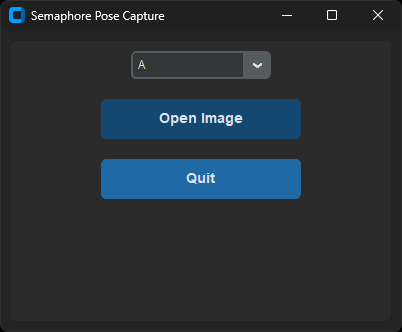
\includegraphics[width=0.7\textwidth]{gui_pose_capture.png}
\end{center}

\subsection{Landmark Pose Semaphore JSON}
\begin{lstlisting}[caption={Contoh File JSON Landmark Pose Semaphore}]
  [
      {
          "pose_landmarks": [
              {
                  "landmark_name": "nose",
                  "x": 0.5,
                  "y": 0.5,
                  "z": 0.5
              },
              {
                  "landmark_name": "left_shoulder",
                  "x": 0.4,
                  "y": 0.4,
                  "z": 0.4
              },
              ...
          ]
      }
  ]
\end{lstlisting}
Selengkapnya bisa dilihat di folder \texttt{semaphore\_poses}.

\subsection{Hasil}
\begin{center}
    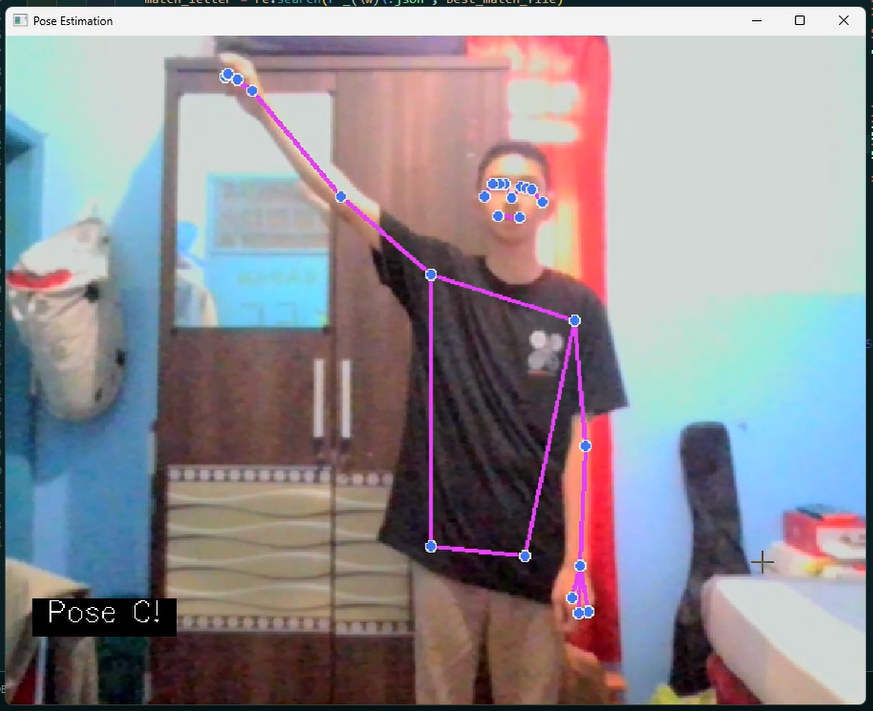
\includegraphics[width=1.0\textwidth]{results_pose.png}
\end{center}

\subsection{Analisis}
Dari hasil yang diperoleh, program berhasil mendeteksi pose tubuh manusia berdasarkan gambar yang diunggah dan membandingkannya dengan data landmark pose yang telah disimpan sebelumnya. Program juga mampu menampilkan pesan yang menunjukkan huruf semaphore yang paling mirip dengan pose yang terdeteksi. Program ini dapat digunakan untuk mengenali pose semaphore dan membandingkan dengan data yang telah disimpan, sehingga dapat membantu dalam analisis dan evaluasi pose semaphore yang dihasilkan. Namun karena masih tahap awal, program ini masih memiliki beberapa kekurangan, seperti sensitivitas terhadap pose yang terdeteksi dan keakuratan dalam membandingkan pose dengan data yang disimpan.

\section{Link Repository GitHub dan Video}
\begin{itemize}
    \item \textbf{Repository GitHub:} \url{https://github.com/rigelra15/semaphore_pose_estimation_opencv.git}
    \item \textbf{Video Demo:} \url{https://youtu.be/bWh0-rXyjdc}
\end{itemize}

\section{Kesimpulan}
\begin{justify}
    Proyek ini berhasil mengimplementasikan deteksi landmark pose manusia berdasarkan pose semaphore menggunakan pustaka MediaPipe. Sistem ini mampu menangkap dan menyimpan data pose untuk setiap huruf semaphore (A-Z) dalam file JSON. Sistem ini juga menyediakan antarmuka pengguna grafis (GUI) yang ramah pengguna dan fungsi untuk menguji dan membandingkan pose semaphore berdasarkan huruf yang telah ditentukan. Sistem ini dapat digunakan untuk analisis dan evaluasi pose semaphore yang dihasilkan.
\end{justify}

\end{document}
